\clearpage
\section{Discussion}

這裏我想討論兩個主題,一個是 accum\-grad 的效果,另一個是 sine linear gamma function 的效果。


\subsection{The effect of accum-grad}

一開始在 review 助教給的 code 的時候,發現這個以前我從來沒有使用過的參數,所以想說來討論一下這個參數的效果。 這裡我使用 32 個 batch 來累積梯度,並且每個 batch 是 32 張圖片,也就是說我的目標是實現 1024 張圖片的訓練的效果。
\begin{figure}[h]
    \centering
    \begin{subfigure}{0.48\textwidth}
        \centering
        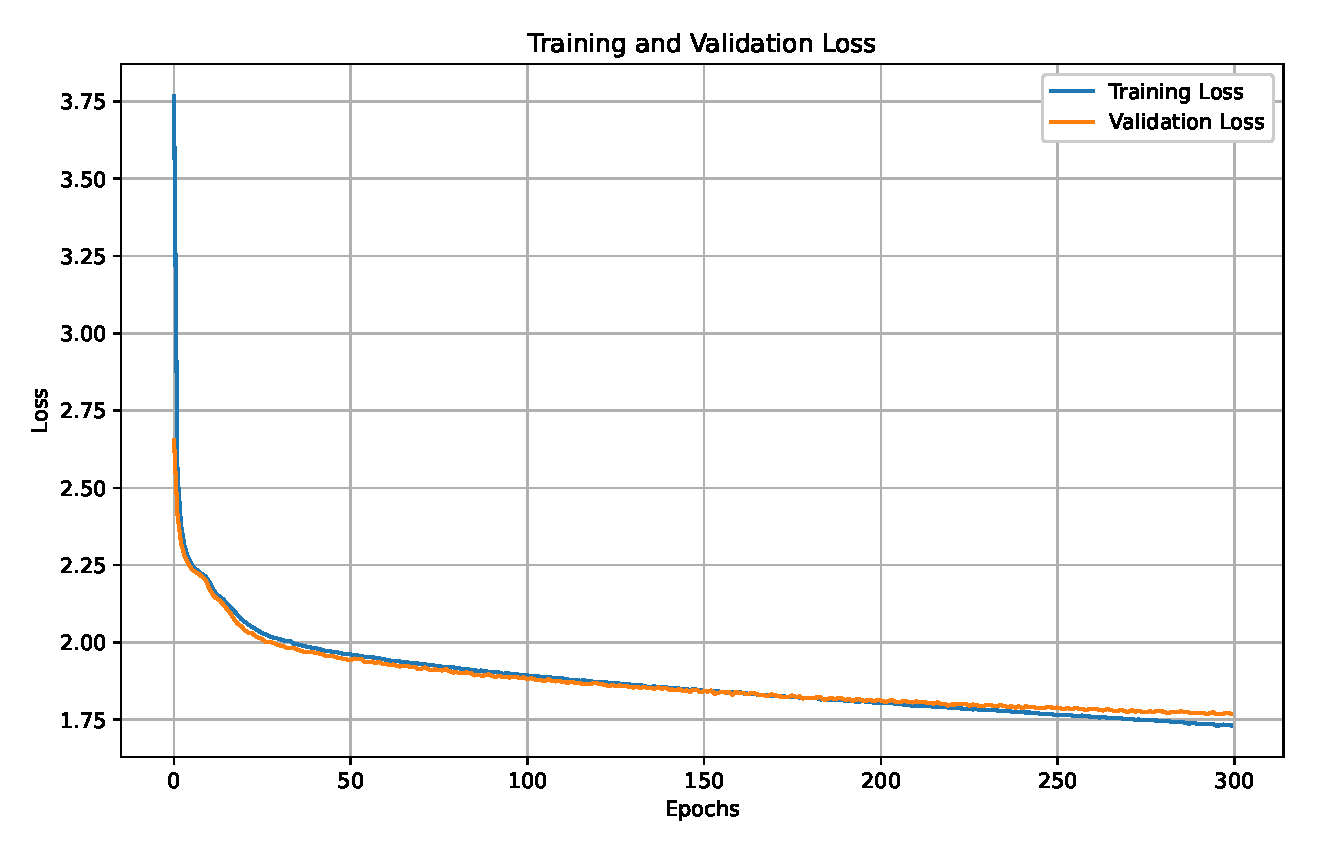
\includegraphics[width=\textwidth]{figures/loss_plot.eps}
        \label{fig:normal_loss_plot}
    \end{subfigure}
    \hfill
    \begin{subfigure}{0.48\textwidth}
        \centering
        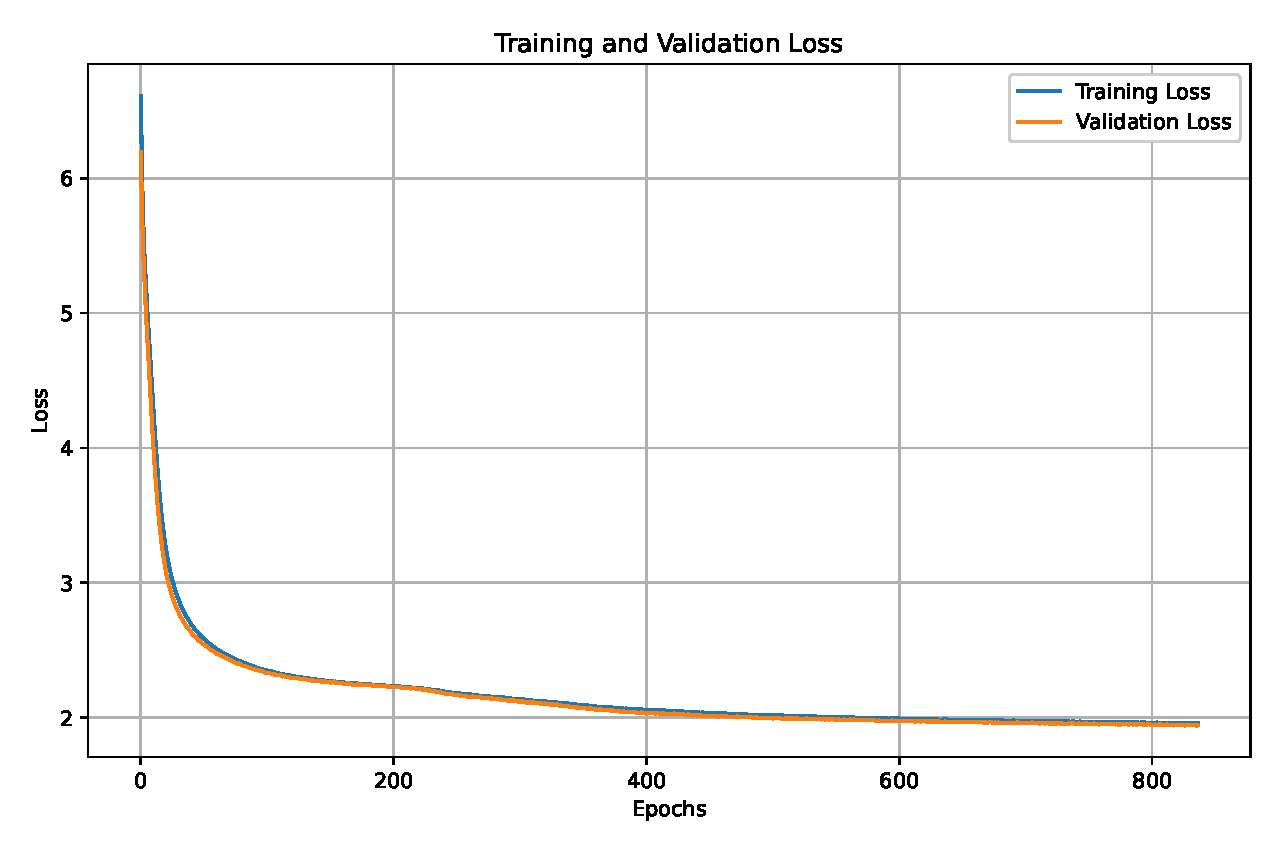
\includegraphics[width=\textwidth]{figures/accum-grad_loss_plot.eps}
        \label{fig:accum-grad_loss_plot}
    \end{subfigure}
    \caption{標準訓練與梯度累積訓練的損失函數對比。左:標準訓練的損失函數;右:梯度累積訓練的損失函數}
    \label{fig:loss_comparison}
\end{figure}

我們可以發現使用 accum-grad 訓練的時候,loss 下降的非常慢,而且最後的結果也不好。 如果對比等效的 epoch 約為 800 / 32 = 25,確實與正常的訓練方式的 Loss 數值在 25 個 epoch 左右差不多。  不過礙於時間有限,這次的實作沒辦法測試當等效 epoch 為 300 時,accum-grad 訓練的結果。 以及這次我用正常的訓練方法到達 300 epoch 時,其實 validation 與 train loss 都還有下降的趨勢,所以我目前的訓練方法其實還有進步的空間。


\begin{figure}[h]
    \centering
    \begin{subfigure}{0.48\textwidth}
        \centering
        \includegraphics[width=\textwidth, height=2.1cm, keepaspectratio]{figures/ag-epoch800-test_69.png}
        \label{fig:ag-epoch800-test_69}
    \end{subfigure}
    \hfill
    \begin{subfigure}{0.48\textwidth}
        \centering
        \includegraphics[width=\textwidth, height=2.1cm, keepaspectratio]{figures/ag-fid-score.png}
        \label{fig:ag-fid-score}
    \end{subfigure}
    \caption{梯度累積訓練的測試結果與 FID 分數。左:梯度累積訓練 800 個 epoch 後的測試結果;右:梯度累積訓練的 FID 分數}
    \label{fig:ag-epoch800-test}
\end{figure}




\subsection{The effect of sine linear gamma function}
這個 sine linear gamma function 是我覺得蠻有趣的設計。 這裡我們來討論一下這個 gamma function 的效果。
首先我們可以發現,對於正常的 linear gamma function,這個方法的表現可以說是非常差,但是其實當模型效果不錯的時候,這個方法的表現跟正常的訓練方法差不多。 所以可以說這個方法可以放大模型的弱勢,但這個方法有什麼用呢? 目前還沒有想法,所以這裡就先不討論了。



\begin{figure}[h]
    \centering
    \includegraphics[width=\textwidth]{figures/fid_comparison_8_12.eps}
    \caption{不同 gamma 函數策略的 FID 分數比較}
    \label{fig:fid_comparison_8_12}
\end{figure}


這裡來觀察 fid score 的凸起,也就是最差的第 45 個 epoch 的結果。

\begin{figure}[h]
    \centering
    \begin{subfigure}{\textwidth}
        \centering
        \includegraphics[width=0.8\textwidth]{figures/test_69.png}
        \label{fig:mask_test_69}
    \end{subfigure}
    % \vspace{1cm}
    \begin{subfigure}{\textwidth}
        \centering
        \includegraphics[width=0.8\textwidth]{figures/bad-linear-test_69.png}
        \label{fig:bad-linear-test_69}
    \end{subfigure}
    % \vspace{1cm}
    \begin{subfigure}{\textwidth}
        \centering
        \includegraphics[width=0.8\textwidth]{figures/bad-sine-linear-test_69.png}
        \label{fig:bad-sine-linear-test_69}
    \end{subfigure}
    \caption{不同 gamma 函數對測試圖像的影響比較。上圖best fid score 的測試圖像;中圖為使用線性 gamma 函數的測試結果;下圖為使用 sine linear gamma 函數的測試結果}
    \label{fig:gamma-comparison-test}
\end{figure}

我覺得除了背景比較雜之外,臉的細節其實還沒不錯的,可以看成是躲在草後面的貓,可能大膽生成的策略對背景生成不友善吧! 或許可以認定凸起的 FID Score 是因為背景的雜訊,所以訓練其實是有正確收斂的。
